\documentclass[]{article}
\usepackage[utf8]{inputenc}
\usepackage{fullpage}
\usepackage[pdftex]{graphicx}
\usepackage{hyperref}

\title{Introduction to Reshaping Data with \texttt{reshape}}
\author{Hadley Wickham. http://had.co.nz/reshape}

\date{2006-02-27}

\begin{document}

\maketitle

\begin{abstract}

Restructuring data is a common task in practical data analysis, and it is usually unintuitive and tedious. Data often has multiple levels of grouping (nested treatments, split plot designs, or repeated measurements) and typically requires investigation at multiple levels. For example, from a long term clinical study we may be interested in investigating relationships over time, or between times or patients or treatments.  Performing these investigations fluently requires the data to be reshaped in different ways.

Currently R supplies a reshape function that can perform some of these tasks, but confounds multiple steps in the process and is hard to use.  We propose a new conceptual framework for reshaping operations and an R package to ``melt'' data frames and then flexibly ``cast'' them to meet your needs. This framework also produces contingency tables, cross-tabulations, and summary statistics.

\end{abstract}

\section{Introduction}

This paper discusses a conceptual framework for data reshaping, and describes an implementation of these principles in an R package, \texttt{reshape}.  

Data reshaping is easiest to define with respect to aggregation.  Aggregation is a common and familiar task where data is reduced and rearranged into a smaller, more convenient form, with a concomitant reduction in the amount of information.  One commonly used aggregation procedure are Excel's Pivot tables.  Reshaping involves a similar rearrangement, but preserves all original information.  Where aggregation reduces many cells in the original data set to one cell in the new dataset, reshaping preserves a one-to-one connection.  

There are a number of general R functions that can aggregate data, for example \texttt{tapply}, \texttt{by} and \texttt{aggregate}, and a function specifically for reshaping data, \texttt{reshape}.  Each of these functions tends to deal well with one or two specific scenarios, and each requires slightly different input arguments.  In practice, careful thought is usually required to piece together the correct sequence of operations to arrange the data how you want.  The \texttt{reshape} package overcomes these problems by using the conceptual framework defined below to solve a general set of problems using just two functions, \texttt{reshape} and \texttt{melt}.  

\section{Conceptual framework}

To help us think about all the ways we might rearrange a data set it is useful to think about data in a somewhat unusual fashion.  Usually, we think about data in terms of a matrix or data frame, where we have observations in the rows and variables in the columns.  In this form it is difficult to investigate relationships between other facets of the data: between subjects, or treatments, or replicates.  Reshaping the data allows us to explore these other relationships while still being able to use the familiar tools that operate on columns.  Reshaping is an important (but often unrecognised) part of practical data analysis and is often necessary when exploring, displaying and analysing data.

For the purposes of reshaping, we can divide the variables into two groups: identifier and measured variables.

\begin{enumerate}
	\item Identifier, or id, variables identify the unit that measurements take place on.  Id variables are usually discrete, and are typically fixed by design.  In ANOVA notation ($Y_ijk$), id variables are the indices on the variables ($i, j, k$).
	\item Measured variables represent what is measured on that unit ($Y$).
\end{enumerate}

It is possible to take this abstraction a step further and say there are only id variables and a value, where the id variables now also identify what measured variable the value represents.  For example, we could represent this table:

\bigskip
\begin{tabular}{|l|r||r|r|r|}\hline
	Subject & Time & Age & Weight & Height \\\hline
	John Smith & 1 & 50 & 90 & 1.80\\\hline
	Mary Smith & 1 & NA & NA & 1.70\\\hline
\end{tabular}

\bigskip
\noindent as:
\bigskip

\begin{tabular}{|l|r|l||r|}\hline
	Subject & Time & Variable & Value \\\hline
	John Smith & 1 & Age & 50 \\\hline
	John Smith & 1 & Height & 90 \\\hline
	John Smith & 1 & Weight & 1.80 \\\hline
	Mary Smith & 1 & Height & 1.7\\\hline
\end{tabular}

\bigskip
\noindent Now each row represents one observation of one variable.  This is what I will refer to as ``melted'' data.  Compared to the original data set, it has a new id variable ``variable'', and a new column ``value'', which represents the value of that observation.  We now have the data in a form in which there is no distinction between our original observed variables and other id variables.  

\section{Implementation}

With this conceptual framework established, I will discuss particular details of the implementation in R.  Ideally, we want easy to use tools to restructure data frames that use the insights from the ideas above.  I will discuss why we need a new package to reshape data, and how we can specify the form of the reshaped data.

The first step is to ``melt'' the data.  This is essentially a trivial operation, and very similar to the existing R function \texttt{stack}.  The next challenge is to specify how we want the data to look with the \texttt{reshape} function.  A natural way to do this is to specify which variables should form the columns and which should form the rows.  In the usual data frame, the ``variable'' id variable forms the columns, while all other id variables form the rows.  Aggregation occurs when the variables do not uniquely identify one row, and in this case we need an aggregation function to reduce the data.  Examples later in the chapter will make this concrete.

The order in which the row and column variables are specified in is very important.  As with a contingency table there are many possible ways of displaying the same variables, and the way they are organised reveals different patterns in the data.  Variables specified first vary slowest, and those specified last vary fastest.  Because comparisons are made most easily between adjacent cells, the variable you are most interested in should be specified last, and the early variables should be thought of as conditioning variables.  An additional constraint is that displays have limited width but essentially infinite length, so variables with many levels must be specified as row variables.  It is also desirable to adhere to common conventions, so where possible, ``variable'' should appear in the column specification.

\subsection{Melting}

The R command to melt a data set is \texttt{melt}.  If you don't specify either measured or id variables, the function will try to guess which are id variables: any factors, integers or columns with 5 or fewer unique values.  If you specify only the measured variables, it assumes the remainder are identifier variables, and vice versa.

One complication of this design is that all values must be of the same type.  This is not usually a big problem because most of the time you are dealing with numeric data.  I have been experimenting with storing this data in a list for maximum flexibility---this however makes later code more complicated as we can no longer rely on straightforward vectorisation.

\subsection{Functions that return multiple values}

Occasionally it is useful to aggregate with a function that returns multiple values, e.g. range, summary etc.  This can be thought of as combining multiple casts each with an aggregation function that returns one variable.  We do this with an additional variable, \texttt{result\_variable} that differentiates the multiple return values.  This \texttt{result\_variable} uses names if available, otherwise will create names of the form X1, X2,\dots  By default, this new id variable will be shown as last column variable, but you can specify the position manually by including \texttt{result\_variable} in the list of row and column variables.

\subsection{Row and column names}

There are two ways to think about the results from an aggregation command, as either a matrix of numbers with some attributes that describe the row and column names, or as a data frame with the row names as columns.  Most current R aggregation functions return the first, implicit, form, whereas cast returns the explicit data frame form.  Why the difference?  The implicit form is often inconvenient to deal with---rownames are data too.

\subsection{Example}


The \texttt{reshape} package is available on CRAN and can be installed using the R command \texttt{install.packages("reshape")}.  This section will work through some techniques using the reshape package with an example data set (\texttt{french\_fries}).  The data is from a sensory experiment investigating the effect of different frying oils on the taste of french fries over time.  There are three different types of frying oils (treatment), each in two different fryers (rep), tested by 12 people (subject) on 10 different days (time).  The sensory attributes recorded, in order of desirability, are potato, buttery, grassy, rancid, painty flavours.  The first few rows of the data look like:

% latex table generated in R 2.2.0 by xtable 1.3-0 package
% Sat Feb 25 11:04:30 2006
\begin{table}[ht]
\begin{center}
\begin{tabular}{rlllrrrrrr}
\hline
 & time & treatment & subject & rep & potato & buttery & grassy & rancid & painty \\
\hline
61 & 1 & 1 & 3 & 1.00 & 2.90 & 0.00 & 0.00 & 0.00 & 5.50 \\
25 & 1 & 1 & 3 & 2.00 & 14.00 & 0.00 & 0.00 & 1.10 & 0.00 \\
62 & 1 & 1 & 10 & 1.00 & 11.00 & 6.40 & 0.00 & 0.00 & 0.00 \\
26 & 1 & 1 & 10 & 2.00 & 9.90 & 5.90 & 2.90 & 2.20 & 0.00 \\
63 & 1 & 1 & 15 & 1.00 & 1.20 & 0.10 & 0.00 & 1.10 & 5.10 \\
27 & 1 & 1 & 15 & 2.00 & 8.80 & 3.00 & 3.60 & 1.50 & 2.30 \\
\hline
\end{tabular}
\end{center}
\end{table}


One of the first things we might be interested in is how balanced this design is, and whether there are many different missing values.  We can investigate this using length as our aggregation function:

\begin{verbatim}
ff_d <- melt(french_fries, id=1:4)
cast(ff_d, subject ~ time, length)

                                      
   time  1  2  3  4  5  6  7  8  9  10
subject X1 X2 X3 X4 X5 X6 X7 X8 X9 X10
      3 30 30 30 30 30 30 30 30 30  NA
     10 30 30 30 30 30 30 30 30 30  30
     15 30 30 30 30 25 30 30 30 30  30
     16 30 30 30 30 30 30 30 29 30  30
     19 30 30 30 30 30 30 30 30 30  30
     31 30 30 30 30 30 30 30 30 NA  30
     51 30 30 30 30 30 30 30 30 30  30
     52 30 30 30 30 30 30 30 30 30  30
     63 30 30 30 30 30 30 30 30 30  30
     78 30 30 30 30 30 30 30 30 30  30
     79 30 30 30 30 30 30 29 28 30  NA
     86 30 30 30 30 30 30 30 30 NA  30
\end{verbatim}

Of course we can also create our own aggregation function.  Each subject should have had 30 observations at each time, so by displaying the difference we can more easily see where the data is missing.

\begin{verbatim}
cast(ff_d, subject ~ time, function(x) 30 - length(x))

                                      
   time  1  2  3  4  5  6  7  8  9  10
subject X1 X2 X3 X4 X5 X6 X7 X8 X9 X10
      3  0  0  0  0  0  0  0  0  0  NA
     10  0  0  0  0  0  0  0  0  0   0
     15  0  0  0  0  5  0  0  0  0   0
     16  0  0  0  0  0  0  0  1  0   0
     19  0  0  0  0  0  0  0  0  0   0
     31  0  0  0  0  0  0  0  0 NA   0
     51  0  0  0  0  0  0  0  0  0   0
     52  0  0  0  0  0  0  0  0  0   0
     63  0  0  0  0  0  0  0  0  0   0
     78  0  0  0  0  0  0  0  0  0   0
     79  0  0  0  0  0  0  1  2  0  NA
     86  0  0  0  0  0  0  0  0 NA   0
\end{verbatim}

We can also easily see the range of values that each variable takes:

\begin{verbatim}
cast(ff_d, variable ~ ., function(x) c(min=min(x), max=max(x)))

                        
result_variable  max min
       variable  max min
        buttery 11.2   0
         grassy 11.1   0
         painty 13.1   0
         potato 14.9   0
         rancid 14.9   0
\end{verbatim}

Since the data is fairly well balanced, we can do some (crude) investigation as to the effects of the different treatments.  For example, we can calculate the overall means for each sensory attribute for each treatment:

\begin{verbatim}
cast(ff_d, treatment ~ variable, mean, 
margins=c("grand_col", "grand_row"))

                                                  
 variable buttery grassy painty potato rancid    .
treatment buttery grassy painty potato rancid    .
        1    1.78  0.649   2.58   6.89   4.07 3.19
        2    1.97  0.663   2.46   7.00   3.62 3.15
        3    1.72  0.681   2.53   6.97   3.87 3.15
        .    1.82  0.664   2.52   6.95   3.85 3.16
\end{verbatim}

Note the row and column margins.  We can also produce margins at different levels.  The following example shows the results broken down for subjects 3 and 11, with both overall means and means for each subject:

\begin{verbatim}
cast(ff_d, treatment + subject ~ variable, mean, 
margins="treatment", subset=subject %in% c(3,10))

                                                      
          variable buttery grassy painty potato rancid
treatment  subject buttery grassy painty potato rancid
        1        3   0.372 0.1889   3.11   6.22   2.11
                10   6.750 0.5850   1.37   9.95   4.02
                 .   3.729 0.3974   2.20   8.18   3.11
        2        3   0.589 0.1056   2.48   6.74   3.14
                10   6.980 0.4750   0.82  10.00   2.15
                 .   3.953 0.3000   1.61   8.45   2.62
        3        3   0.767 0.0944   2.87   5.29   2.86
                10   6.450 0.1450   0.69  10.03   3.11
                 .   3.758 0.1211   1.72   7.79   2.99
\end{verbatim}

Finally, since we have a repetition over treatments, we might be interested in how reliable each subject is: are the scores for the two reps highly correlated?  We can explore this graphically by reshaping the data and using a lattice plot.  Our graphical tools work best when the things we want to compare are in different columns, so we'll cast the data to have a column for each rep.

\texttt{xyplot(X1 ~ X2 | variable, cast(ff\_d, ... ~ rep), aspect="iso")}

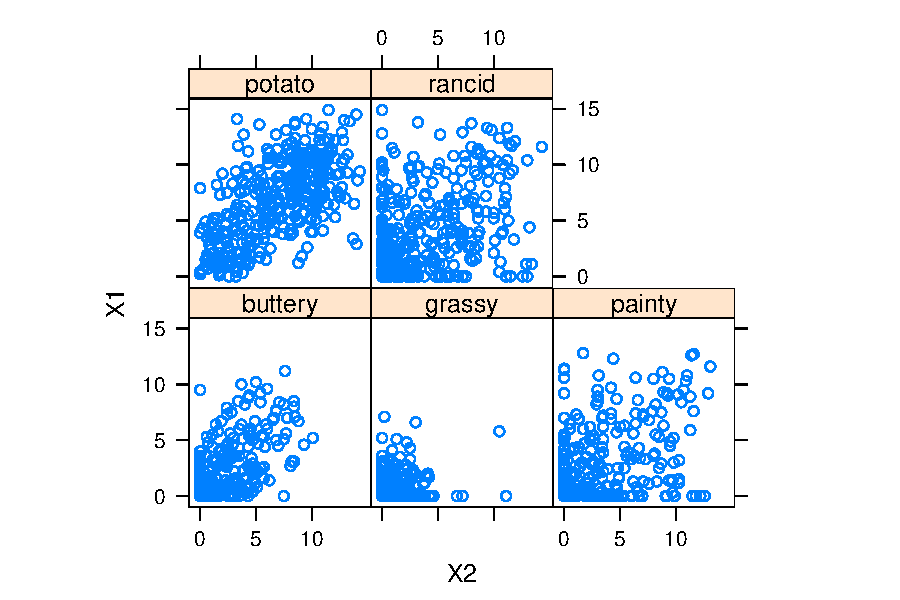
\includegraphics{.introductionw.wcache/1doig.pdf}

If we wanted to explore the relationships between subjects or times or treatments we could follow similar steps.

\section{Where to go next}

Now that you've read this introduction, you should be able to get started using \texttt{reshape}.  I have tried to include lots of examples in the documentation, so if you get stuck have a look at those.  The best places to start are \texttt{?melt} and \texttt{?cast}.  If you have a problem and just can't figure out what's going wrong, please feel free to email me, \href{mailto:h.wickham@gmail.com}{h.wickham@gmail.com}.  I'd also love to hear your comments or any ideas that would make \texttt{reshape} better.

\end{document}

